\section{Methodology and main activities developed}

This section describes the methodology adopted during the internship, which includes iterative development, communication and collaboration tools, stakeholders and their responsibilities, and the activities that were carried out during the internship.

\subsection{Methodology used}
The internship was conducted based on an iterative development approach, characterized by the definition of daily objectives and the execution of activities in the laboratory environment. At the end of each day, feedback was received from the supervisor, which enabled continuous adjustments and improvements in the work developed.

Additionally, some tasks were performed outside laboratorial hours, with the purpose of continuing the project's progress. These activities included specific adjustments to previously developed tasks, documentation of developed solutions (e.g., UML diagrams), and conducting complementary research related to the topic.

Throughout the day, an average of three main briefings were held. The first took place in the morning, with the objective of conducting a project status update, providing feedback on work possibly developed during the week, and defining the main objectives to be achieved during the day. The second briefing occurred at the beginning of the afternoon, when the progress of activities carried out during the morning was discussed. The last briefing was held at the end of the day, with the purpose of reviewing the tasks performed and planning the next project stages for the following week. In this briefing, complementary work to be carried out outside internship hours was also defined.

The supervisor was always available to offer support and clarifications, both during in-person days at the laboratory and outside laboratorial hours, through different communication channels.

In more technical cases or those requiring deeper analysis, there was also always the possibility of consulting other laboratory engineers, who were always available to help.

All communication within the laboratory was conducted in person. In cases where remote communication was necessary, the institutional email was used as the official means.

Since the project covered different areas of knowledge (electronics and computer science), communication was fundamental for aligning expectations and tracking work progress. Throughout the internship, all established requirements were continuously adjusted to meet both the institution’s needs and the intern’s expectations. In this way, the entire project was developed collaboratively and adaptively, ensuring that the goals were achieved effectively.

All code developed during the internship was initially stored in a personal GitHub repository, and later shared with the team through a GitLab repository.

\subsection{Stakeholders, roles and responsibilities}
This internship involved collaboration from different participants, each with specific responsibilities:

\begin{itemize}
    \item Institution supervisor:
    \begin{itemize}
        \item[-] Engineer Pedro Pascoal: Responsible for guiding the intern through continuous supervision and providing constructive feedback regarding the work developed. Also assisted in integrating the intern into the institution's facilities.
    \end{itemize}
    \item FEUP/FCUP tutor:
    \begin{itemize}
        \item[-] Professor Rolando Martins: Responsible for guiding the intern from the academic side, representing the curricular unit's objectives and in preparing the final report.
    \end{itemize}
    \item Client:
    \begin{itemize}
        \item[-] Engineer Pedro Pascoal: Responsible for representing INESC TEC's interests, establishing project requirements and expectations. Also responsible for validating the work developed.
    \end{itemize}
    \item Intern:
    \begin{itemize}
        \item[-] Vasco Melo: Responsible for developing the different tasks proposed by the client, taking into account the quality and time proposed for their completion. Also responsible for reporting the entire internship through the different evaluation elements proposed by the curricular unit.
    \end{itemize}
\end{itemize}

\subsection{Activities developed}

During the internship, different activities were developed, which included project planning, market research, and prototype development. As new requirements emerged, activities were adjusted to meet the project's new demands. Thus, the activities developed can be described as follows:

\begin{itemize}
    \item[] 1. Project planning and market research:
        \begin{itemize}
            \item[.] Introduction of the intern to the facilities and their equipment;
            \item[.] Establishment of an action plan for project development;
            \item[.] Market research was conducted based on available equipment and expected objectives, which were being established/adjusted throughout the project.
        \end{itemize}
    \item[] 2. Raspberry Pi 3 and DS18B20 Sensors:
        \begin{itemize}
            \item[.] Raspberry Pi 3 configuration;
            \item[.] Development of a data reading system with DS18B20 sensors.
        \end{itemize}
    \item[] 3. Creation of a GUI and communication system between the RPI and the MainPC: 
        \begin{itemize}
            \item[.] Requirements gathering for the graphical interface and market technologies;
            \item[.] Development of different prototypes for the GUI;
            \item[.] Establishment of an SSL/TLS protocol with the RPI;
            \item[.] Creation of the temperature test protocol structure with the Raspberry Pi 3 and the MainPC.
        \end{itemize}
    \item[] 4. Set up a management system for test storage:
        \begin{itemize}
            \item[.] Study on data to be stored;
            \item[.] Creation of the database schema;
            \item[.] Implementation of a database control system.
        \end{itemize}
    \item[] 5. Implementation of a database migration system:
        \begin{itemize}
            \item [.] Creation of a database migration system between the MainPC and the RPI;
            \item [.] Creation of a database migration system between the RPI and the EVSE.
        \end{itemize}
    \item[] 6. Communication with the EVSE:
        \begin{itemize}
            \item[.] Establishment of SSH communication between the RPI and the EVSE.
        \end{itemize}
    \item[] 7. Create a dashboard for data visualization:
        \begin{itemize}
            \item[.] Study on dashboard requirements and functionalities;
            \item[.] Analysis of available technologies for implementation;
            \item[.] Testing of different technologies;
            \item[.] Dashboard implementation with defined functionalities.
        \end{itemize}
    \item[] 8. Test migration scheduling system: 
        \begin{itemize}
            \item[.] Establishment of a scheduling system between the MainPC and the RPI;
            \item[.] Establishment of a scheduling system between the RPI and the EVSE.
        \end{itemize}
    \item[] 9.  Communication with the thermal chamber and stabilization detection system:
        \begin{itemize}
            \item[.] Study on thermal chamber functionalities;
            \item[.] Establishment of communication between the RPI and the thermal chamber via serial port;
            \item[.] Investigation of different mathematical formulations for thermal chamber temperature stabilization detection;
            \item[.] Implementation of a temperature stabilization detection system with the thermal chamber.
        \end{itemize}
    \item[] 10. Documentation:
        \begin{itemize}
            \item[.] Elaboration of different UML diagrams for the developed system;
            \item[.] Creation of technical documentation for the developed system.
        \end{itemize}
    \item[] 11. Bootstrapping:
        \begin{itemize}
            \item[.] Elaboration of a dockerfile to facilitate the installation of the MainPC component;
            \item[.] Elaboration of an ansible system to facilitate the installation of the RPI component.
        \end{itemize}
\end{itemize}

For better organization of the work developed, a Gantt chart was elaborated, which can be seen in Figure \ref{fig:gantt_chart}.

\begin{figure}[H]
    \centering
    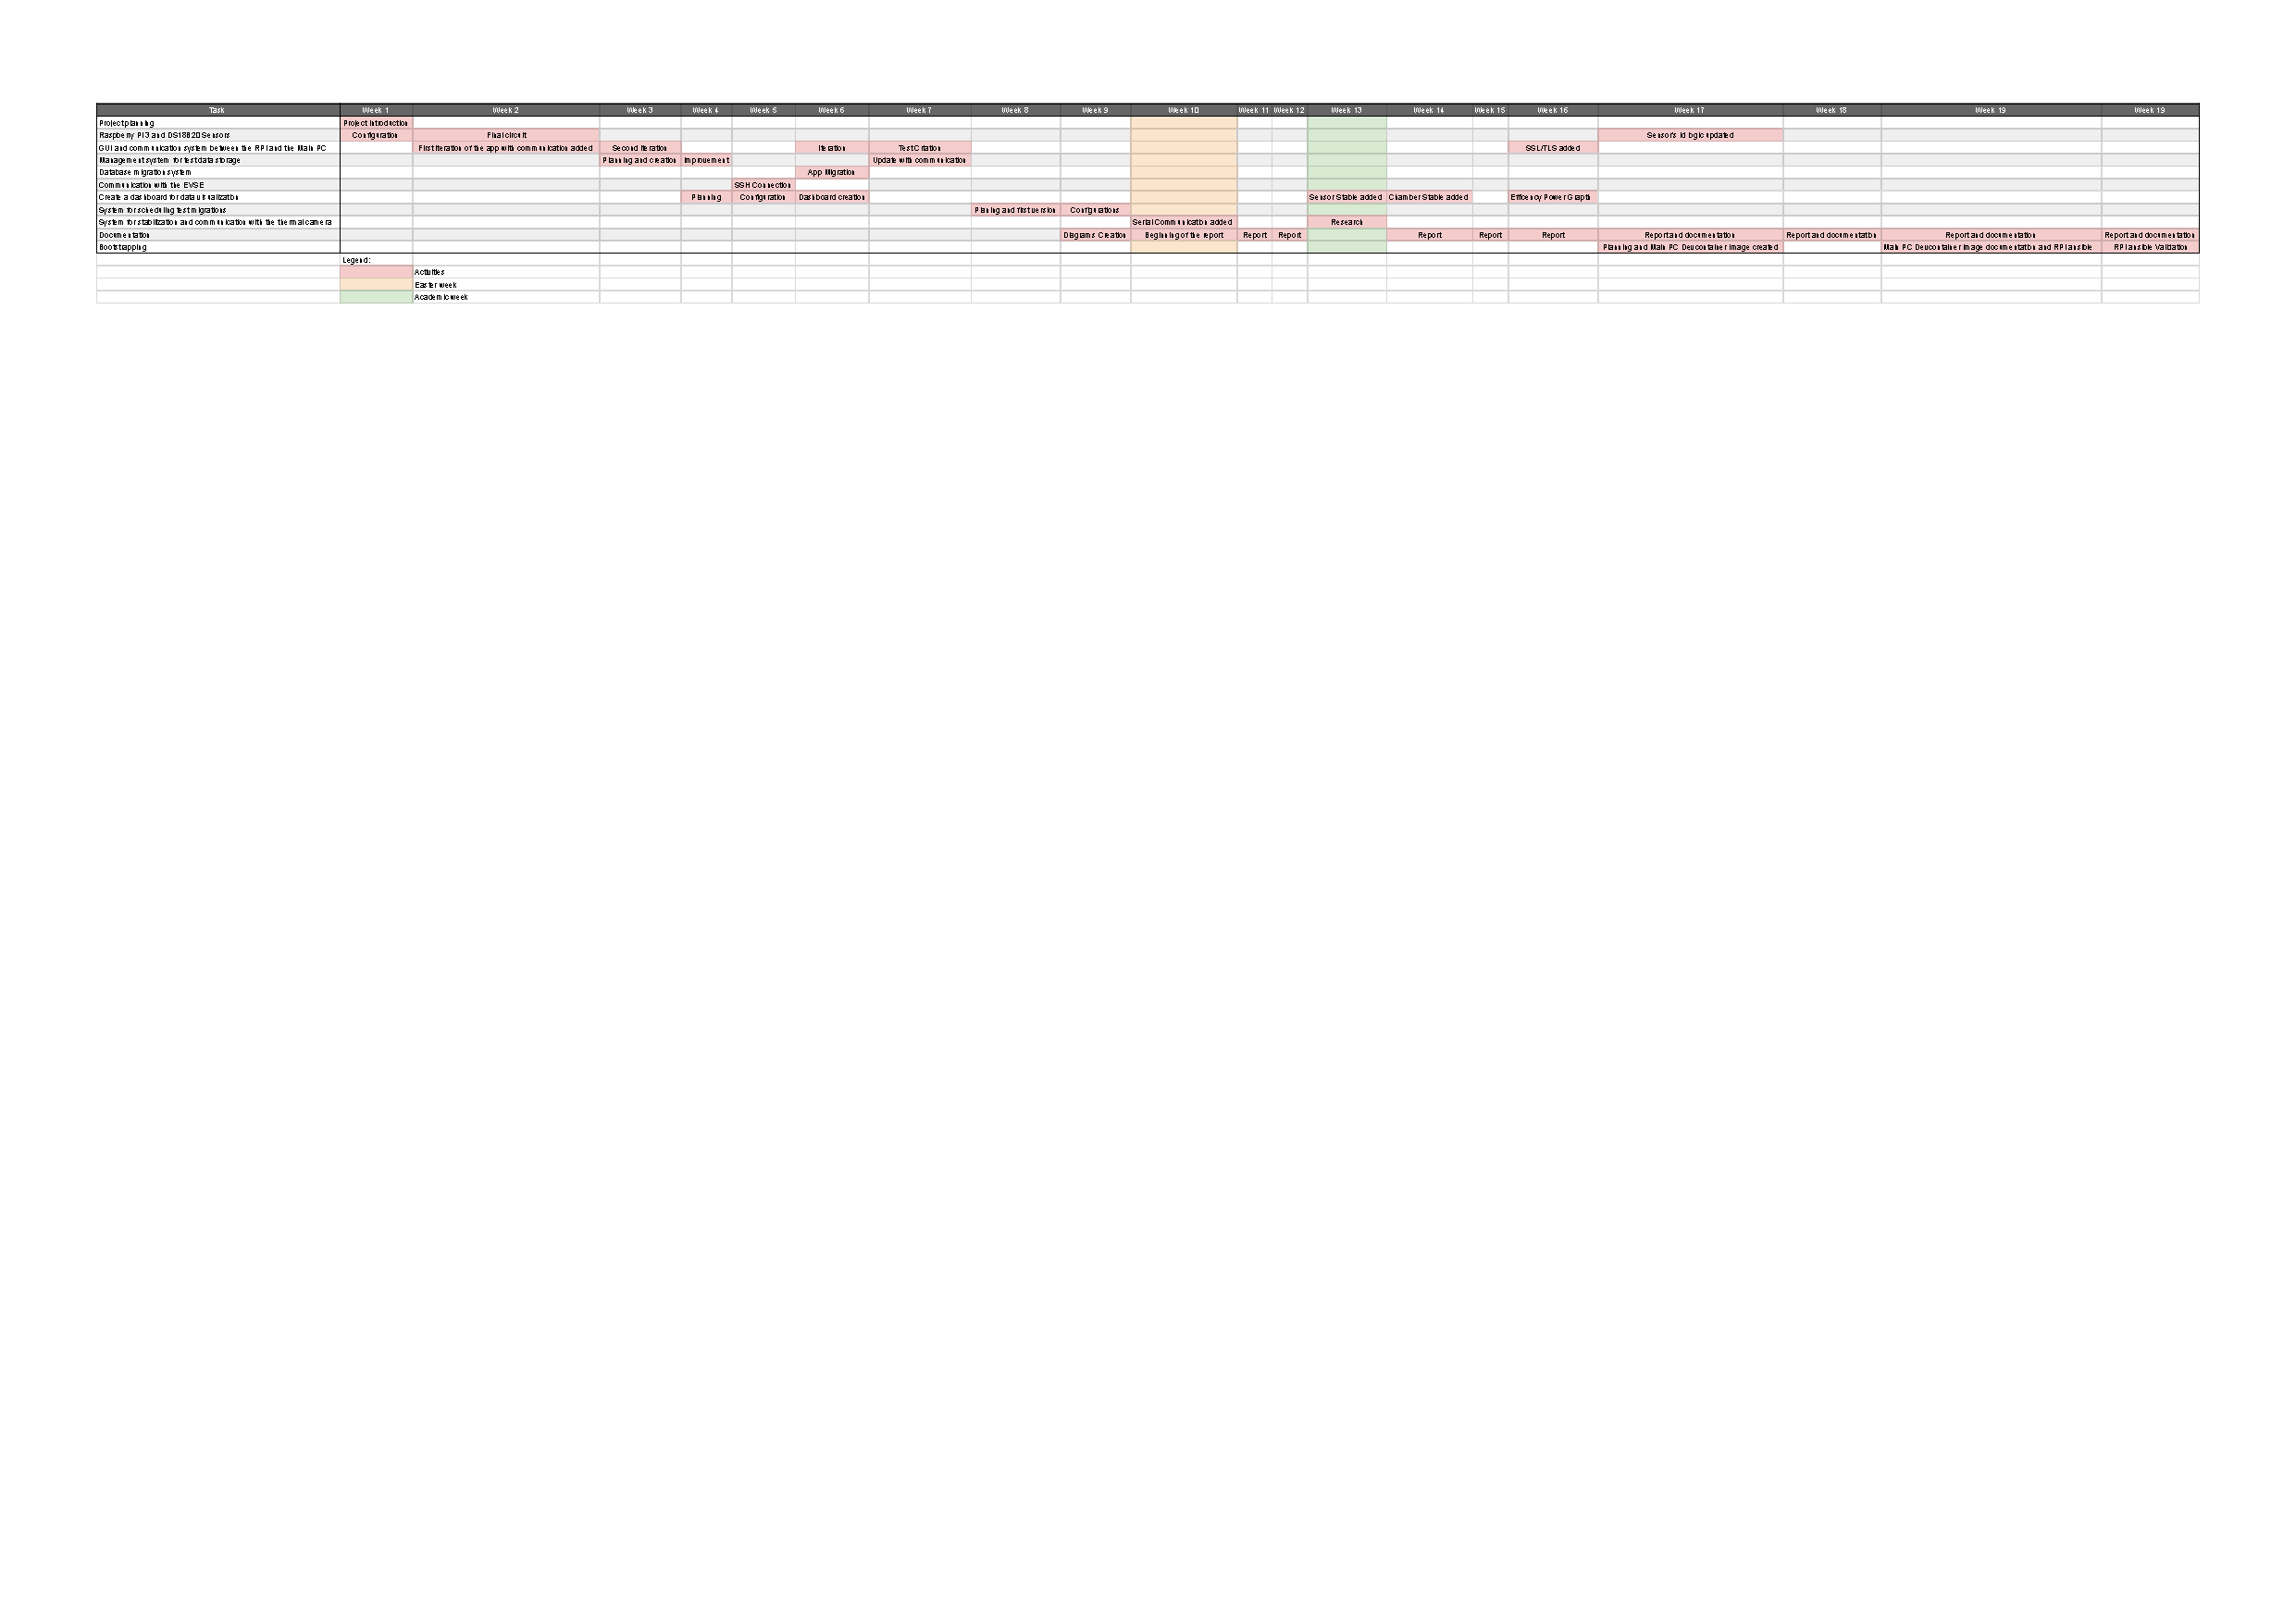
\includegraphics[width=\textwidth, clip, trim=0 24cm 0 0]{figures/ganttchart.pdf}
    \caption{Gantt chart for project tasks}
    \label{fig:gantt_chart}
\end{figure}
